\chapter[Systematic Uncertanties and Statistical Formalism][Systematic Uncertainties and Statistical Formalism]{Systematic Uncertanties and Statistical Formalism}
\label{chapter:systematics} 

This chapter summarizes the various systematic uncertainties that enter the measurement of the limit of \tth multi-lepton analysis, as well as structure of the statistical 
analysis model used to obtain the measurement. The systematic uncertanties arise
from three main sources. The first are the normalization uncertainties on the background process estimation methods, which are discussed in depth in \chapter{backgrounds}. 
The second source is the theoretical uncertainties on the \tth production cross-section and acceptance. The final source are the experiemental and detector related systematic
uncertanties related to event selection efficicienies and measurements and identification of the objects. They affect only the non-data driven backgrounds and the \tth
signal, as simulation is used to model their acceptance and efficiency for the analyiss selection. 

These systematic uncertanties, the estimated background and signal event counts in each of the signal regions, and the observed data in each signal region are combined
in a statistical fit to an analysis model to extract the measurement of interest. We measure per-channel and combined ratios of the observed production rate to the 
theoretically predicted production rate of \tth, a parameter called $\mu$. In the absence of a statistically significan observation, this measurement is translated into a upper confidence limit
on $\mu$. The details of this procedure are discussed in the following sections and the results with the observed data are discussed in Chapter \ref{chapter:results}

\section{Systematic Uncertainties on Signal Cross-section and Acceptance}

The \ttH signal is simulated with matrix elements at NLO (next-to-leading order) in QCD with {\sc Powhel} and is discussed in Chapter \chapter{data}.  

The production cross section and the Higgs boson decay branching fractions together with their theoretical uncertainties from the QCD scale and PDF choice are taken from the NLO theoretical calculations reported in Ref.~\cite{Heinemeyer:2013tqa}. The uncertainty from the QCD scale estimated by varying $\mu_{0}$ by a factor of 2 from the nominal value is $^{+3.8\%}_{-9.3\%}$, while the uncertainty from the PDF set and the value of $\alpha_{\rm S}$ is $\pm 8.1\%$.\\

The impact of the choice of the QCD scale on the simulation of the \ttbar$H$ event selection efficiency is estimated in two independent ways. 

First, the factorisation and renormalisation scales $\mu_{0}$ are varied by a factor of 2, as $\mu = 2\mu_{0}$ and $\mu = \mu_{0}/2$. The effects of these new scales are estimated via the application of event reweighting procedures on the nominal simulation using kinematic distributions at parton level. The weights used are dependent on the transverse momenta of both the \ttbar$H$ system and of the top quark, as described in Ref.~\cite{Guindon:1638000}. 

Second, the choice of the factorisation and renormalisation scales, dependent on fixed (``static'') parameters in the nominal simulation, is tested comparing its prediction with an alternative (``dynamic''), but still physics motivated choice $\mu_{0} = (m_{T}^{t}m_{T}^{\bar{t}}m_{T}^{H})^{\frac{1}{3}}$, which depends on kinematic variables. This comparison is performed via event reweighting of the nominal static simulation based on weights derived as a function of the \ttbar$H$ transverse momentum~\cite{Guindon:1638000}. In order to take the difference between the choices of scale as systematic uncertainties, a symmetric envelope around the nominal simulation is built applying the weights and also their inverses.

Fig.~\ref{fig:theosyst} shows the impact of the different choices for the factorization and renormalization scales on the jet and b-jet multiplicities in events with 2 SS leptons. Similar variations are seen also in the other event categories. In order to not double-count the variations on the total cross section the predictions from the different QCD scales are normalised to the same total cross section. That means that the observed differences are only coming from the event selection.
\begin{figure}[htbp]
\begin{center}
%\begin{subfigure}[t]{0.55\textwidth}
\subfigure[jet multiplicity]{\label{fig:theosyst:a}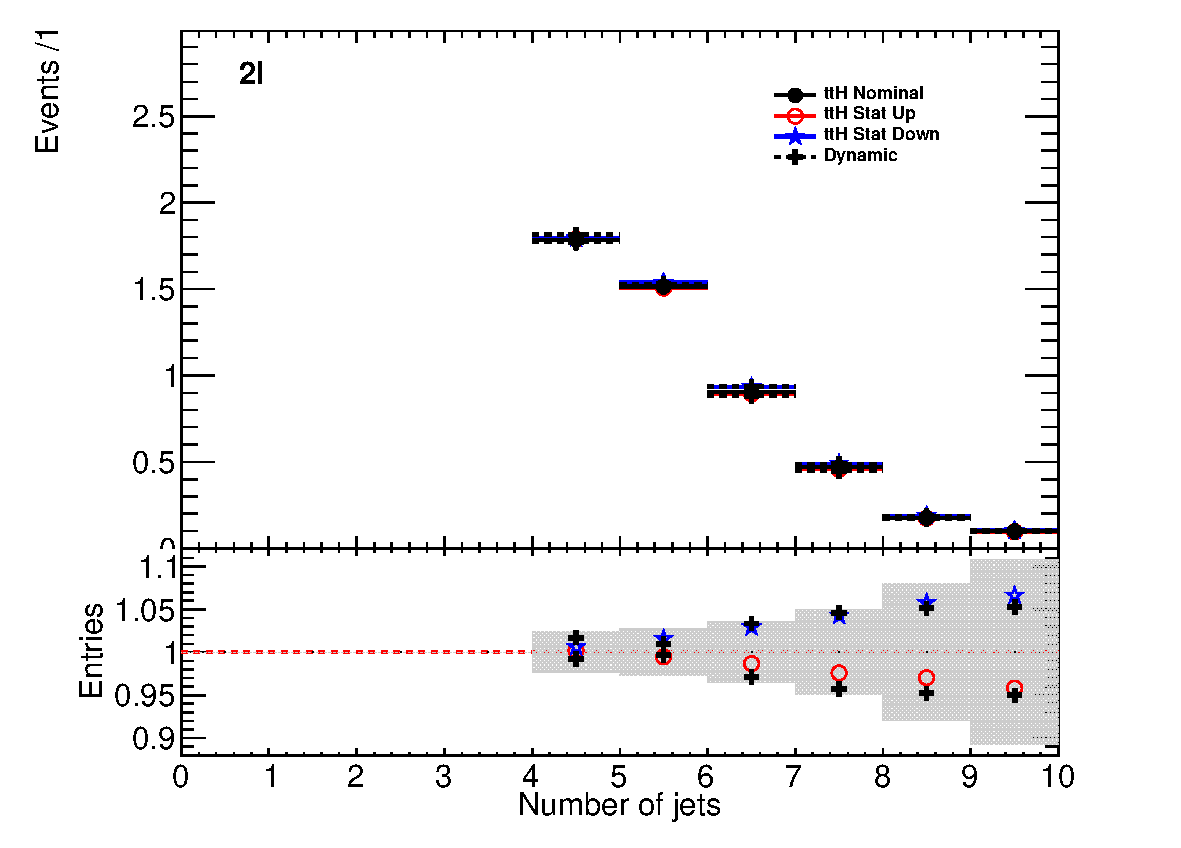
\includegraphics[width=0.48\textwidth]{Figures/Theory/plot_2l_NJet_ttH_nom.eps}}
\subfigure[b-jet multiplicity]{\label{fig:theosyst:b}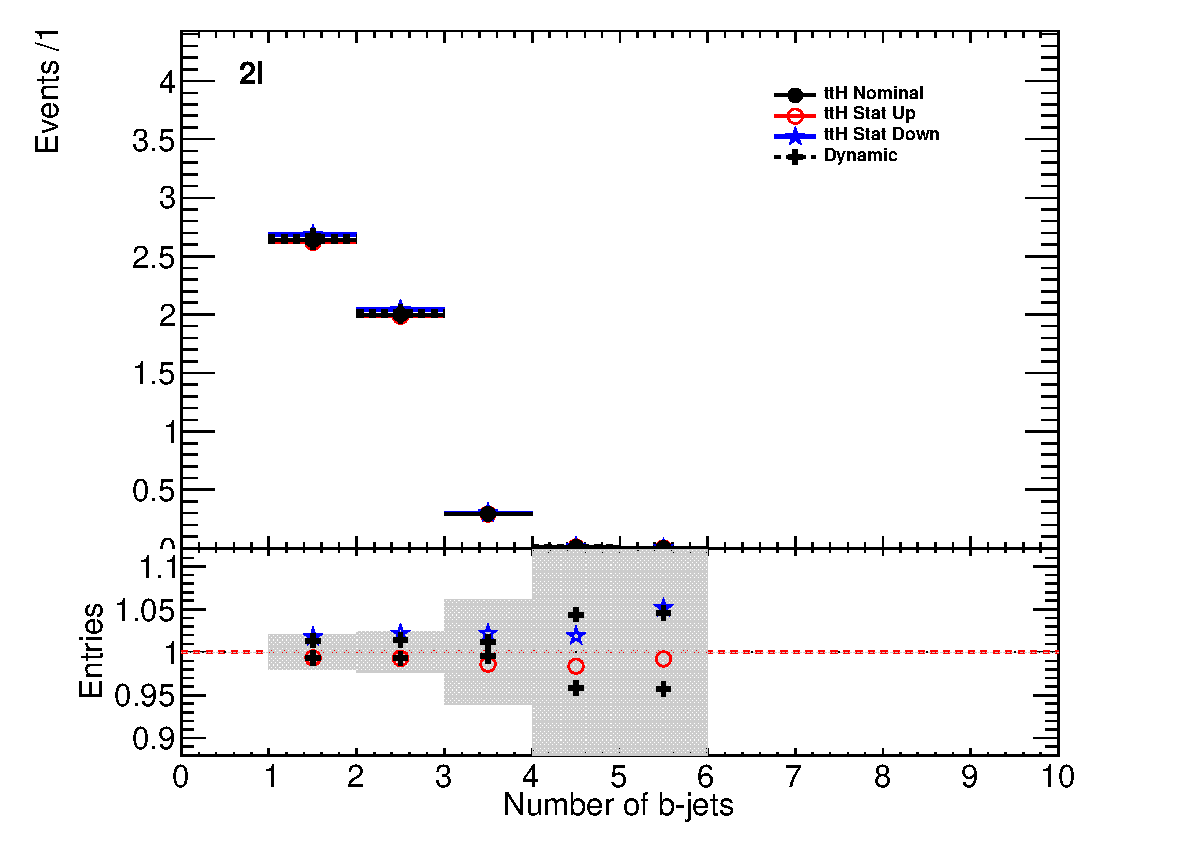
\includegraphics[width=0.48\textwidth]{Figures/Theory/plot_2l_NJetBTag_ttH_nom.eps}}
\caption{Effects on the jet multiplicities in 2 SS lepton \ttbar$H$ events from different choices of the factorization and renormalization scales. ``Static'' refers to the variations by a factor of 2 of the nominal $\mu_{0}$, while ``Dynamic'' refers to the alternative choice of $\mu_{0}$ which depends on the event kinematic. The grey band in the lower panels represents the statistical uncertainty of the nominal sample.}
\label{fig:theosyst}
\end{center}
\end{figure}
Significant variations on the jet multiplicities can be seen and these translate into different predictions on the signal event yields in the signal regions. 
%once the requirements on the minimum number of jets are applied. 
Such differences, listed in Table~\ref{tab:theosystttH}, are taken as theoretical systematic uncertainties in addition to the ones affecting the total \ttbar$H$ production cross section. The ``Static'' uncertainties come from the variations by a factor of 2 from the nominal scale and they are correlated with the uncertainties on the total cross section, which are estimated with the same procedure. The ``Dynamic''  uncertainties come from the difference between the nominal and the alternative dynamic scale and are treated as an independent source of theoretical uncertainty. 

\begin{tabular}{r|c|c|c|c|c|c|}
QCD scale [\%] & 1l\_2tau & 2l4jets & 2l$\geq$5jets & 2l\_tau & 3l & 4l \\
\hline
Static  & $^{+0.7}_{-0.1}$ & $^{+0.6}_{-0.0}$ & $^{+2.7}_{-1.3}$ & $^{+2.7}_{-1.0}$ & $^{+2.3}_{-0.8}$ & $^{+0.9}_{-0.2}$ \\
Dynamic & $^{+0.6}_{-0.0}$ & $^{+1.7}_{-0.8}$ & $^{+2.0}_{-2.6}$ & $^{+1.7}_{-1.1}$ & $^{+1.7}_{-1.1}$ & $^{+0.5}_{-0.0}$ \\
\hline
\end{tabular}
\end{center}
\label{tab:theosystttH}
\end{table}%

The uncertainty of the \ttbar$H$ event selection due to the PDF sets is estimated comparing the predictions with three different PDF sets, varying each set within errors and taking the width of the envelope as systematic uncertainty. The recommended sets are \verb+CT10+, \verb+MSTW2008nlo68cl+ and \verb+NNPDF21_100+. 
We determine the change in the acceptance due to the PDF sets via the formula \ref{Eq:PDFunc} to disentangle it from the change in production cross section.
%\[ \left(\frac{\textrm{Reweighted yield in SR}}{\textrm{Reweighted total
%    number of events}}\right)\left(\frac{\textrm{Original yield in SR}}{\textrm{Original total
%    number of events}}\right)^{-1} \]
\begin{equation} \label{Eq:PDFunc}
\left(\frac{\textrm{Reweighted yield in SR}}{\textrm{Reweighted total number of events}}\right)\left(\frac{\textrm{Original yield in SR}}{\textrm{Original total number of events}}\right)^{-1}-1
\end{equation}
Fig.~\ref{fig:theosystPDF} shows the estimated PDF systematic uncertainties as a function of the jet multiplicity in \ttbar$H$ events with at least two leptons. The uncertainties are compatible with the uncertainty on the production cross section estimated in Ref.~\cite{Heinemeyer:2013tqa} and indicated by the dashed red lines in the lower panel. 
Table \ref{tab:pdfaccttH} shows the half-width of the envelope of the acceptance under all eigenvector variations of the three PDF sets.
No significant dependence on the event topology is observed, so that the PDF systematic uncertainty on the \ttbar$H$ event selection is neglected.
\begin{figure}[htbp]
\begin{center}
%\begin{subfigure}[t]{0.55\textwidth}
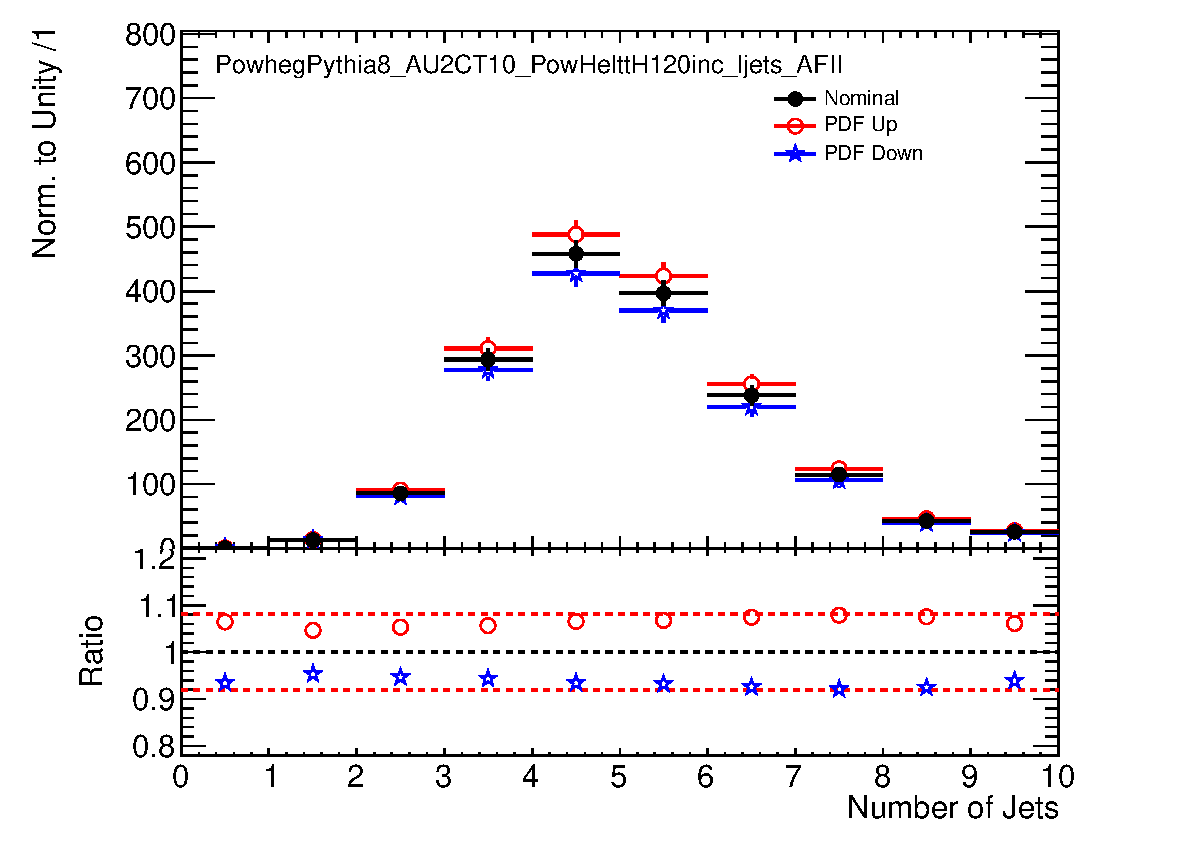
\includegraphics[width=0.6\textwidth]{Figures/Theory/plot_PowhegPythia8_AU2CT10_PowHelttH120inc_ljets_AFII_njets_all_njets_all.eps}
\caption{PDF systematic uncertainty on the jet multiplicities in \ttbar$H$ events with at least 2 leptons. The dashed red lines in the lower panel indicate the systematic uncertainty on the \ttbar$H$ production cross section.}
\label{fig:theosystPDF}
\end{center}
\end{figure}
\begin{table}
\begin{center}
\caption{\label{tab:pdfaccttH}Uncertainties on $\ttbar H$ acceptance in signal
  regions due to PDF variation.}
\begin{tabular}{r|c|c|c|c|c|c}
Sample & 1l\_2tau & 2l 4j & 2l 5j & 2l\_tau & 3l & 4l\\
\hline
$\ttbar H$ & 1.0\% & 0.3\% & 1.0\% & 0.9\% & 0.5\% & 1.4\%\\
\end{tabular}
\end{center}
\end{table}




\section{Summary of Background Systematic Uncertainties}


\section{Summary of Experimental and Detector Systematic Uncertainties}


